This chapter presents the results of the object detection experiments. In the first part of the chapter, the testing setup and the average precision (AP) of the models are presented. Additionally, a few representative models were examined to assess how much performance can vary, to explain the observed irregularities, and to further illustrate the effect of synthetic and real images. In the second part of the chapter, the confidence threshold of the YOLOv8n base model and the best-performing fine-tuned model is optimized to maximize the F1-score, and the detections of both models are qualitatively inspected.

\section{Testing setup and Impact of Synthetic Images}

The testing dataset consisted of 746 images collected from scenarios different from those used in training and validation to ensure that model performance was evaluated on unseen data. The models were evaluated using the Ultralytics Python library to generate predictions on the test images. The evaluation metric AP\textsubscript{IoU:0.50} was computed with the Object Detection Metrics toolkit \cite{electronics10030279}, following the Pascal VOC evaluation standard. Predictions were made using an IoU threshold of 0.5 and a confidence threshold of 0.001 to ensure that confidence filtering would not distort the AP computation. Figure~\ref{fig:detection_results} shows the AP values for the YOLOv8n base model and all models trained with different combinations of real and synthetic images.

\begin{figure}[htbp]
    \centering
    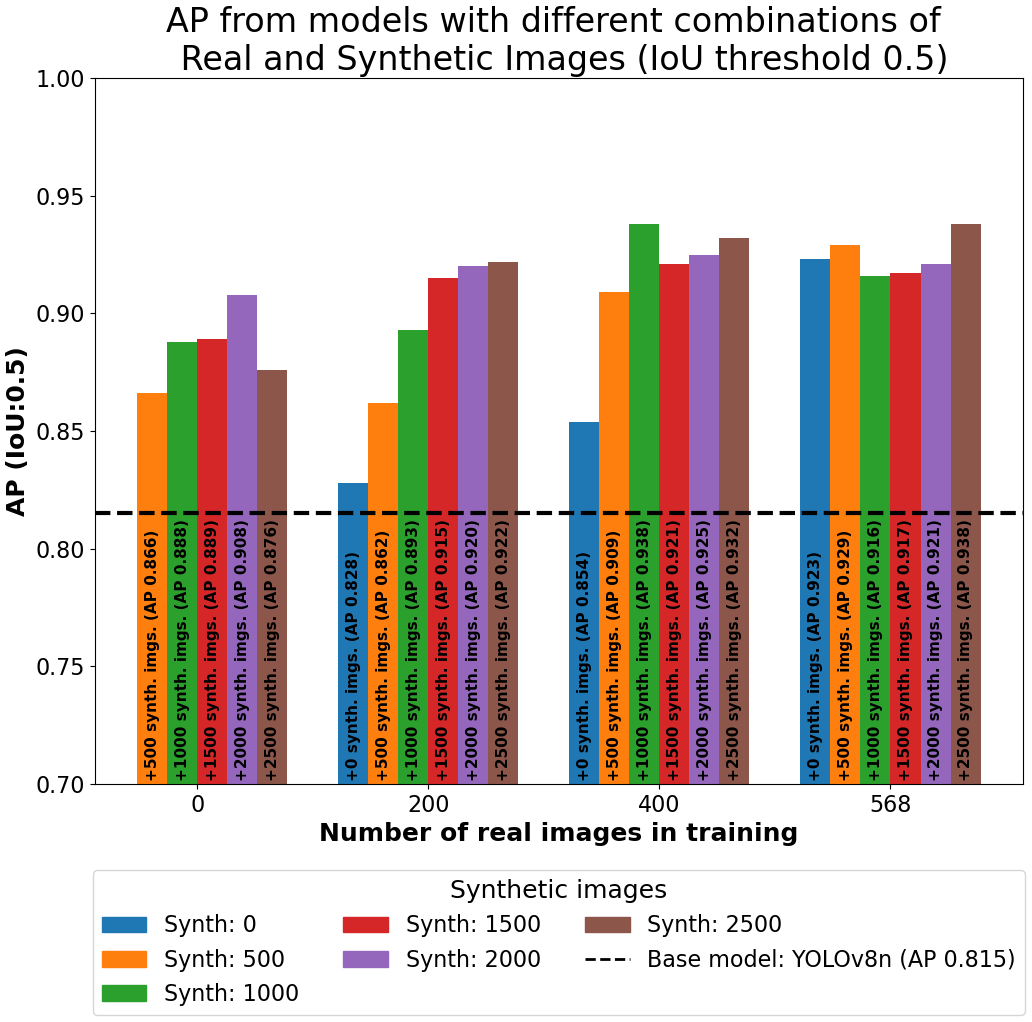
\includegraphics[width=1\textwidth]{images/results/map3.PNG}
    \caption{Average Precision (AP\textsubscript{IoU:0.50}) for the YOLOv8n base model and fine-tuned models trained with different real/synthetic ratios. Exact values are presented inside the bars.}
   \label{fig:detection_results}
\end{figure}

As a general trend, model performance increased with the number of synthetic training images and when real images were added on top of them. Synthetic data alone improved the base model's ability to detect people in real images. The best-performing models were r400s1000 (400 real + 1000 synthetic) and r568s2500, both achieving an AP of 0.938.\footnote{Although both achieve the same AP, the text refers to r568s2500 as the best performing model because it achieved the highest F1-score at the optimized confidence threshold described later (Table~\ref{tab:object_detection_metrics}).}  The YOLOv8n base model performed the weakest, with an AP of 0.815.

Although models trained solely with synthetic data improved their performance, adding real images had a strong positive impact on detection accuracy. For instance, increasing the dataset with 200 real images improved and stabilized the AP of models trained with at least 1500 synthetic images (real images making up approximately 10\% of the dataset). However, this effect was less clear for models trained exclusively on real images. The relatively weak performance of r200 is somewhat surprising, given that adding 200 real images improved and stabilized the models with many synthetic images. Moreover, because the performance of r200 and r400 appeared to follow a logarithmic trend as the dataset size increased, which is typical in deep learning, r568 was expected to achieve an AP similar to s500. Instead, r568 achieved an irregularly high AP.
Due to these irregularities, it is difficult to precisely quantify this effect.

The following irregularities were observed across model configurations:

\begin{itemize}
\item The s2500 model performed second worst among the synthetic-only models, but improved greatly in mixed datasets.
\item r200s500 performed worse than s500.
\item r400s1000 achieved a highest AP together with r568s2500.
\item r568 showed a sudden increase compared to r200 and r400 models.
\item r568s500 was the second-best performer in the r568 group, contrary to the general trend.
\end{itemize}

While hyperparameters were kept constant across all trainings, even small changes in dataset composition affected the learning process, as seen in Figure~\ref{fig:detection_results}. To better understand the underlying causes of the observed performance variations, an additional experiment was conducted after obtaining the main results to assess the effect of stochasticity in deep learning training. First, the training process was verified to be deterministic when using the same dataset and seed, as retraining produced identical weights. Then, three models, namely s2500, r568, and r568s2500, were each retrained twice using different but shared random seeds. The following AP means and standard deviations in Table~\ref{tab:ap50_seed_stats} were obtained across the original and retrained models:

\begin{table}[htbp]
    \caption{AP\textsubscript{IoU:0.50} mean and standard deviation across three runs of models trained with different shared seeds.}
\label{tab:ap50_seed_stats}
\centering
\renewcommand{\arraystretch}{1.15}
\setlength{\tabcolsep}{8pt}
\begin{tabular}{|c|r|c|}
\hline
\multirow{2}{*}{Model} & \multicolumn{2}{c|}{AP\textsubscript{IoU:0.50}} \\ \cline{2-3}
                       & Mean & Standard deviation \\ \hline
s2500       & 0.886 & 	0.010 \\ \hline
r568        & 0.900 & 	0.027 \\ \hline
r568s2500   & 0.932 & 	0.010 \\ \hline
\end{tabular}
\end{table}

These results indicate that random initialization can have a notable effect on model performance, which partly explains why some models outperform or underperform relative to expectations. This is particularly evident in the case of the r568 model, where the standard deviation is high and the mean AP is considerably lower than that shown in Figure~\ref{fig:detection_results}. Similar irregularities related to random seed selection were also observed when retraining once the r400s1000 and r400s1500 models. In the original results (Figure~\ref{fig:detection_results}), r400s1000 (AP 0.938) outperformed r400s1500 (AP 0.921), whereas after retraining with a new shared seed, the relationship was reversed (r400s1000: AP 0.930, r400s1500: AP 0.932). This further confirms that stochastic variations during training can significantly alter the relative ranking of models with otherwise similar data compositions (especially for small datasets).

Beyond the stochastic effects, the results in Table~\ref{tab:ap50_seed_stats} also highlight how dataset itself influence both the stability and performance of the model. The s2500 model achieved a lower mean AP than r568, while the r568 model exhibited nearly three times higher standard deviation. When these datasets were combined in the r568s2500 model, both the mean AP improved significantly and the standard deviation decreased to the level of s2500.

\section{Confidence Threshold Optimization and Qualitative Analysis}

To find the optimal confidence threshold that produces the highest F1-score, scikit-learn's \texttt{precision\_recall\_curve} function was used. Before providing inputs to the function, predictions were filtered with an IoU threshold of 0.5. As described in Section~\ref{sec:object_detection_evaluation_metrics}, the precision-recall curve is obtained by plotting precision and recall for each confidence threshold. To identify the optimal confidence threshold, F1-scores were computed using Equation~\ref{eq:f1} and plotted against the corresponding confidence thresholds. The threshold that yielded the highest F1-score was selected. Figures~\ref{fig:threshold} show F1-scores for different confidence thresholds for the YOLOv8n base model and the r568s2500 model:

\begin{figure}[htbp]
    \centering
    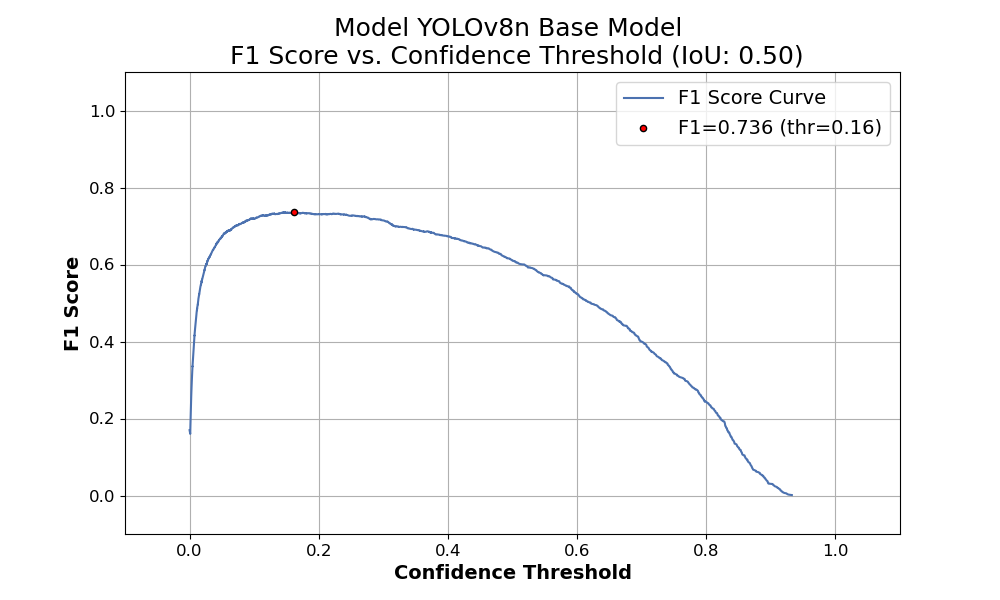
\includegraphics[width=0.8\textwidth]{images/results/yolo_base_f1_scores_0_50.png}
    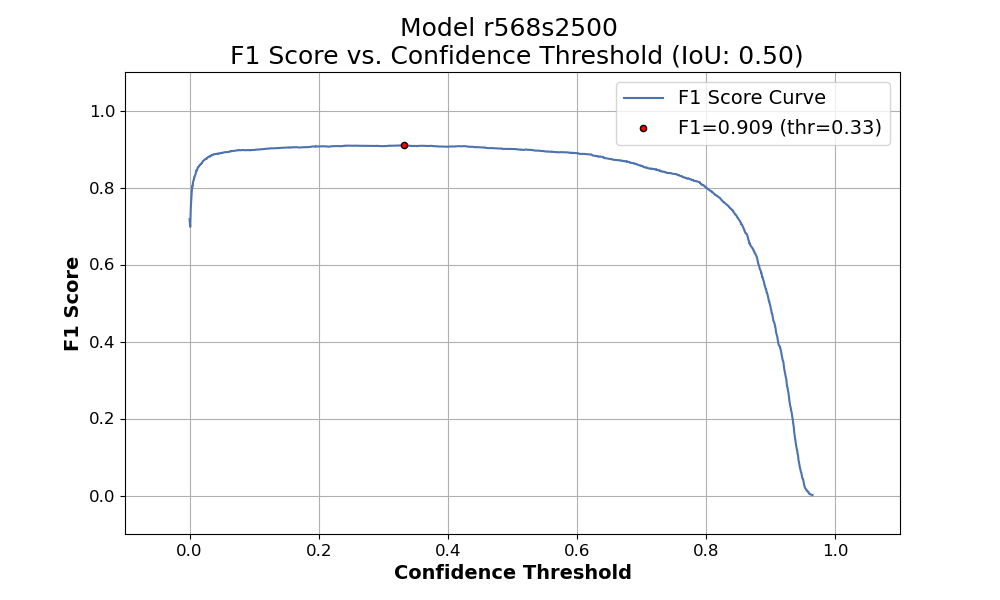
\includegraphics[width=0.8\textwidth]{images/results/r568_s2500_f1_scores_0_50.png}
    \caption{F1-scores over all confidence thresholds for the YOLOv8n base model and the r568s2500 model. The highest F1-score on the curve is marked with a dot.}
    \label{fig:threshold}
\end{figure}

From the plots in Figure~\ref{fig:threshold}, it can be seen that the YOLOv8n base model reaches its highest F1-score (F1 = 0.736) at a confidence threshold of 0.16, while the r568s2500 model reaches its maximum (F1 = 0.909) at a threshold of 0.33. A lower F1-score indicates weaker overall performance, which can result from low precision, low recall or both. The figures also show that the YOLOv8n model maintains a high F1-score within the range of 0.10-0.20 before it starts to decline relatively steadily, whereas the r568s2500 model maintains high performance between 0.10-0.50 and drops sharply after 0.80. As mentioned in Section~\ref{sec:object_detection_evaluation_metrics}, a higher confidence threshold results in more false negatives (and fewer false positives) as predictions are discarded under stricter criteria. Based on this, it can be concluded that the YOLOv8n base model detects people across a broad range of confidence levels, as its F1-score starts to decline steadily after a confidence threshold of 0.20. In contrast, the r568s2500 model produces consistently high-confidence detections, maintaining a strong F1-score until a sharp drop occurs beyond 0.80. This indicates that discarding predictions above this threshold rapidly disrupts the balance between precision and recall. The s2500 model, trained solely on synthetic data, also exhibited a similar F1-score curve to the r568s2500 model, as shown in Appendix~\ref{fig:s2500_f1_scores_0_50}.

A more detailed quantitative overview of the model predictions is presented in Table~\ref{tab:selected_models_counts}, which summarizes the number of ground-truth objects, total predictions, true positives (TP), false positives (FP), and false negatives (FN) for the selected models using optimized confidence thresholds and an IoU threshold of 0.5.

\begin{table}[htbp]
    \caption{Ground truth, predictions, true positives (TP), false positives (FP), and false negatives (FN) for the YOLOv8n base model and r568s2500 model using optimized confidence thresholds.}
\label{tab:selected_models_counts}
\centering
\renewcommand{\arraystretch}{1.15}
\setlength{\tabcolsep}{8pt}
\begin{tabular}{|l|r|r|r|r|r|}
\hline
Model & Ground-truth & Predictions & TP & FP & FN \\ \hline
YOLOv8n    & 1785 & 1496 & 1207 & 289 & 578 \\ \hline
r568s2500  & 1785 & 1714 & 1591 & 123 & 194 \\ \hline
\end{tabular}
\end{table}

From the Table~\ref{tab:selected_models_counts}, it can be observed that the YOLOv8n base model produced the largest number of false detections, both FP and FN. After fine-tuning with real and synthetic data, the number of false negatives decreased by approximately two-thirds compared to the base model, and false positives were reduced by more than half. For all models presented in Figure~\ref{fig:detection_results}, the optimized confidence thresholds and related evaluation metrics are provided in Table~\ref{tab:object_detection_metrics}. An interesting observation from  the previously mentioned table is that the r200 and r400 models had false positive values in the range of around 400 at their selected confidence thresholds, which is notably higher than that of the YOLOv8n base model.

\vspace{5pt}
\noindent
\textbf{YOLOv8n base model:}  
A qualitative inspection of the YOLOv8n predictions (Figure~\ref{fig:yolov8n_tp} and \ref{fig:yolov8n_fnfp}) showed that the model performs reliably in straightforward scenarios where a 

\begin{figure}[!htbp]
\centering
% Row 1
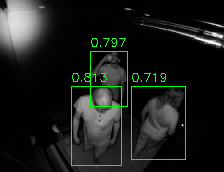
\includegraphics[width=0.32\textwidth]{images/results/yolov8n/onnistuneet/royale_20240710_110402_frame198.png}
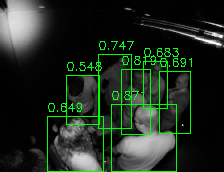
\includegraphics[width=0.32\textwidth]{images/results/yolov8n/onnistuneet/royale_20240710_110908_frame147.png}
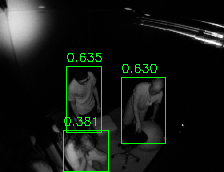
\includegraphics[width=0.32\textwidth]{images/results/yolov8n/onnistuneet/royale_20240710_110908_frame261.png}\\[4pt]
% Row 2
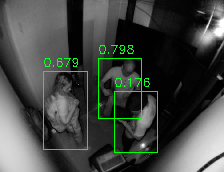
\includegraphics[width=0.32\textwidth]{images/results/yolov8n/onnistuneet/royale_20240710_130444_frame327.png}
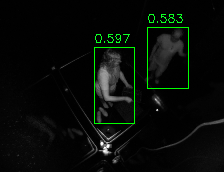
\includegraphics[width=0.32\textwidth]{images/results/yolov8n/onnistuneet/royale_20240710_134224_frame1098.png}
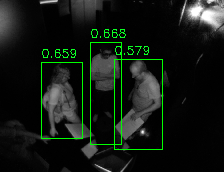
\includegraphics[width=0.32\textwidth]{images/results/yolov8n/onnistuneet/royale_20240710_141816_frame519.png}
\caption{Examples of successful detections by the YOLOv8n base model. Green bounding boxes indicate detected persons, with confidence scores shown above each box.}
\label{fig:yolov8n_tp}
\end{figure}

\begin{figure}[htbp]
\centering
% Row 1
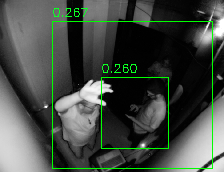
\includegraphics[width=0.32\textwidth]{images/results/yolov8n/virhe/royale_20240710_130444_frame549.png}
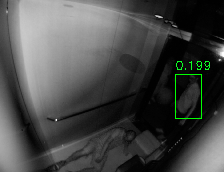
\includegraphics[width=0.32\textwidth]{images/results/yolov8n/virhe/royale_20240710_113404_frame387.png}
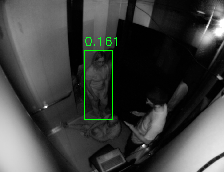
\includegraphics[width=0.32\textwidth]{images/results/yolov8n/virhe/royale_20240710_130444_frame201.png}\\[4pt]
% Row 2
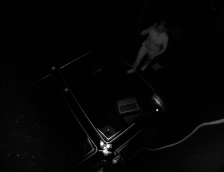
\includegraphics[width=0.32\textwidth]{images/results/yolov8n/virhe/royale_20240710_134224_frame1071.png}
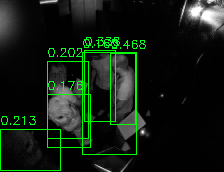
\includegraphics[width=0.32\textwidth]{images/results/yolov8n/virhe/royale_20240710_141816_frame690.png}
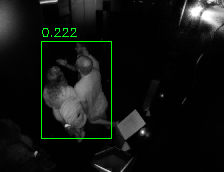
\includegraphics[width=0.32\textwidth]{images/results/yolov8n/virhe/royale_20240710_141816_frame747.png}
\caption{Examples of detections by the YOLOv8n base model, showing both false negatives and false positives.}
\label{fig:yolov8n_fnfp}
\end{figure}

person is clearly visible and upright. The model was also capable of detecting close-range human figures without major difficulties. However, it often failed to detect people in more complex settings, such as partially occluded individuals, those positioned near doorways, or persons lying on the floor. Especially in images with bright lighting, strong reflections, or shadows (as seen in the upper images of Figure~\ref{fig:yolov8n_fnfp}), people were frequently not detected at all. These undetected cases constituted the majority of false negatives.
False positives were frequently caused by the model interpreting parts of the environment (e.g., furniture or bags) as humans, especially when these objects overlapped or resembled human silhouettes. In several cases, large regions of the environment were incorrectly classified as people.

\vspace{5pt}
\noindent
\textbf{Fine-tuned model (r568s2500):}  
The fine-tuned model r568s2500 demonstrated a clear improvement in both recall and precision. Visual inspection confirmed that the fine-tuned model was able to detect nearly all standard cases where a person was visible, even under challenging lighting and viewing conditions. The model also avoided mistaking environmental structures for humans. By comparing Figures~\ref{fig:yolov8n_tp} and \ref{fig:r568s2500_tp}, it can be seen that the fine-tuned model successfully detected people in corresponding cases while the confidence levels were generally higher. False negatives occasionally occurred in extreme cases, such as individuals lying down, standing behind a door in a dark area, or being partially occluded. The improved performance can be clearly seen by comparing Figures~\ref{fig:yolov8n_fnfp} and \ref{fig:fine_fnfp}. However, unlike the YOLOv8n base model, in cases where individuals interacted closely with the camera or prominently raised their hands, the model often detected the hands as separate persons, as shown in Figure~\ref{fig:fine_kasi}. This accounted for most of the false positive cases. Notably, this phenomenon of misclassifying hands as people occurred across all fine-tuned models, including those trained purely on real or synthetic data. This strongly suggests that the cause of this issue lies in the way training data were labeled.

%\vspace{60pt}

\begin{figure}[!htbp]
\centering
% Row 1
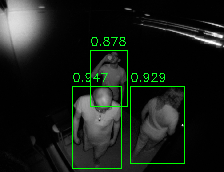
\includegraphics[width=0.32\textwidth]{images/results/r568s2500/onnistuneet/royale_20240710_110402_frame198.png}
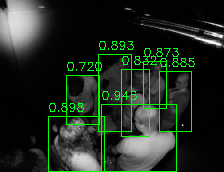
\includegraphics[width=0.32\textwidth]{images/results/r568s2500/onnistuneet/royale_20240710_110908_frame147.png}
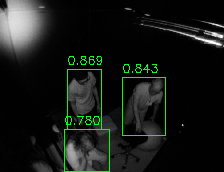
\includegraphics[width=0.32\textwidth]{images/results/r568s2500/onnistuneet/royale_20240710_110908_frame261.png}\\[4pt]
% Row 2
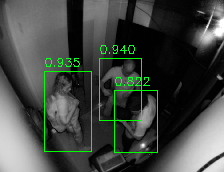
\includegraphics[width=0.32\textwidth]{images/results/r568s2500/onnistuneet/royale_20240710_130444_frame327.png}
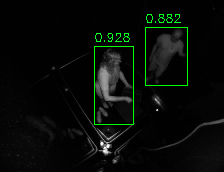
\includegraphics[width=0.32\textwidth]{images/results/r568s2500/onnistuneet/royale_20240710_134224_frame1098.png}
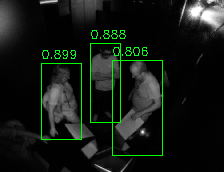
\includegraphics[width=0.32\textwidth]{images/results/r568s2500/onnistuneet/royale_20240710_141816_frame519.png}
\caption{Detections of the r568s2500 model for the corresponding images shown in Figure~\ref{fig:yolov8n_tp}.}
\label{fig:r568s2500_tp}
\end{figure}

\begin{figure}[ht]
\centering
% Row 1
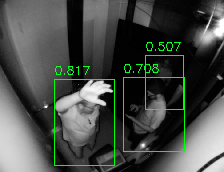
\includegraphics[width=0.32\textwidth]{images/results/r568s2500/compare/royale_20240710_130444_frame549.png}
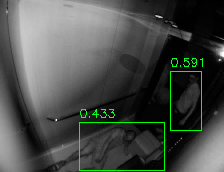
\includegraphics[width=0.32\textwidth]{images/results/r568s2500/compare/royale_20240710_113404_frame387.png}
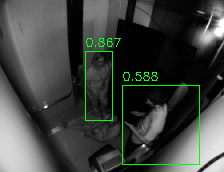
\includegraphics[width=0.32\textwidth]{images/results/r568s2500/compare/royale_20240710_130444_frame201.png}\\[4pt]
% Row 2
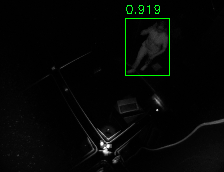
\includegraphics[width=0.32\textwidth]{images/results/r568s2500/compare/royale_20240710_134224_frame1071.png}
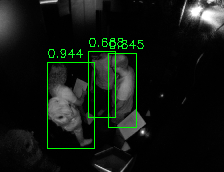
\includegraphics[width=0.32\textwidth]{images/results/r568s2500/compare/royale_20240710_141816_frame690.png}
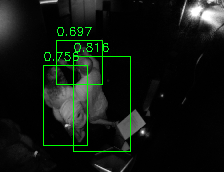
\includegraphics[width=0.32\textwidth]{images/results/r568s2500/compare/royale_20240710_141816_frame747.png}
\caption{Detections of the r568s2500 model for the corresponding images shown in Figure~\ref{fig:yolov8n_fnfp}.}
\label{fig:fine_fnfp}
\end{figure}

\begin{figure}[ht]
\centering
% Row 1
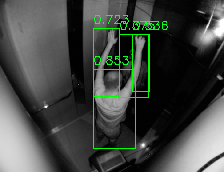
\includegraphics[width=0.49\textwidth]{images/results/r568s2500/kasi/royale_20240710_130444_frame909.png}
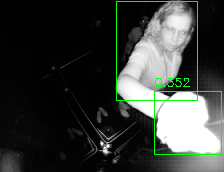
\includegraphics[width=0.49\textwidth]{images/results/r568s2500/kasi/royale_20240710_134224_frame1146.png}
\caption{Examples of false positive cases detected by the r568s2500 model, where hands were occasionally detected as separate persons.}
\label{fig:fine_kasi}
\end{figure}

In summary, the qualitative and quantitative analyses consistently show that fine-tuning the YOLOv8n base model with both real and synthetic images greatly improved its robustness across diverse indoor scenarios. When comparing the YOLOv8n base model to the best-performing r568s2500 model, AP increased from 0.815 to 0.938 (+0.123, ~15\%). The peak F1-score rose from 0.736 to 0.909 (+0.173, ~24\%) and at the optimized thresholds false negatives decreased from 578 to 194 (~66\% reduction) while false positives dropped from 289 to 123 (~57\% reduction).